\clearpage

\renewcommand{\tablename}{Supplementary Table}
\setcounter{table}{0}

%\begin{table}
%\caption{Comparison of Top 10\% Depleted Genes with Hart \textit{et al}. Fitness Genes with Bayes Factor (BF).}
%\centering
%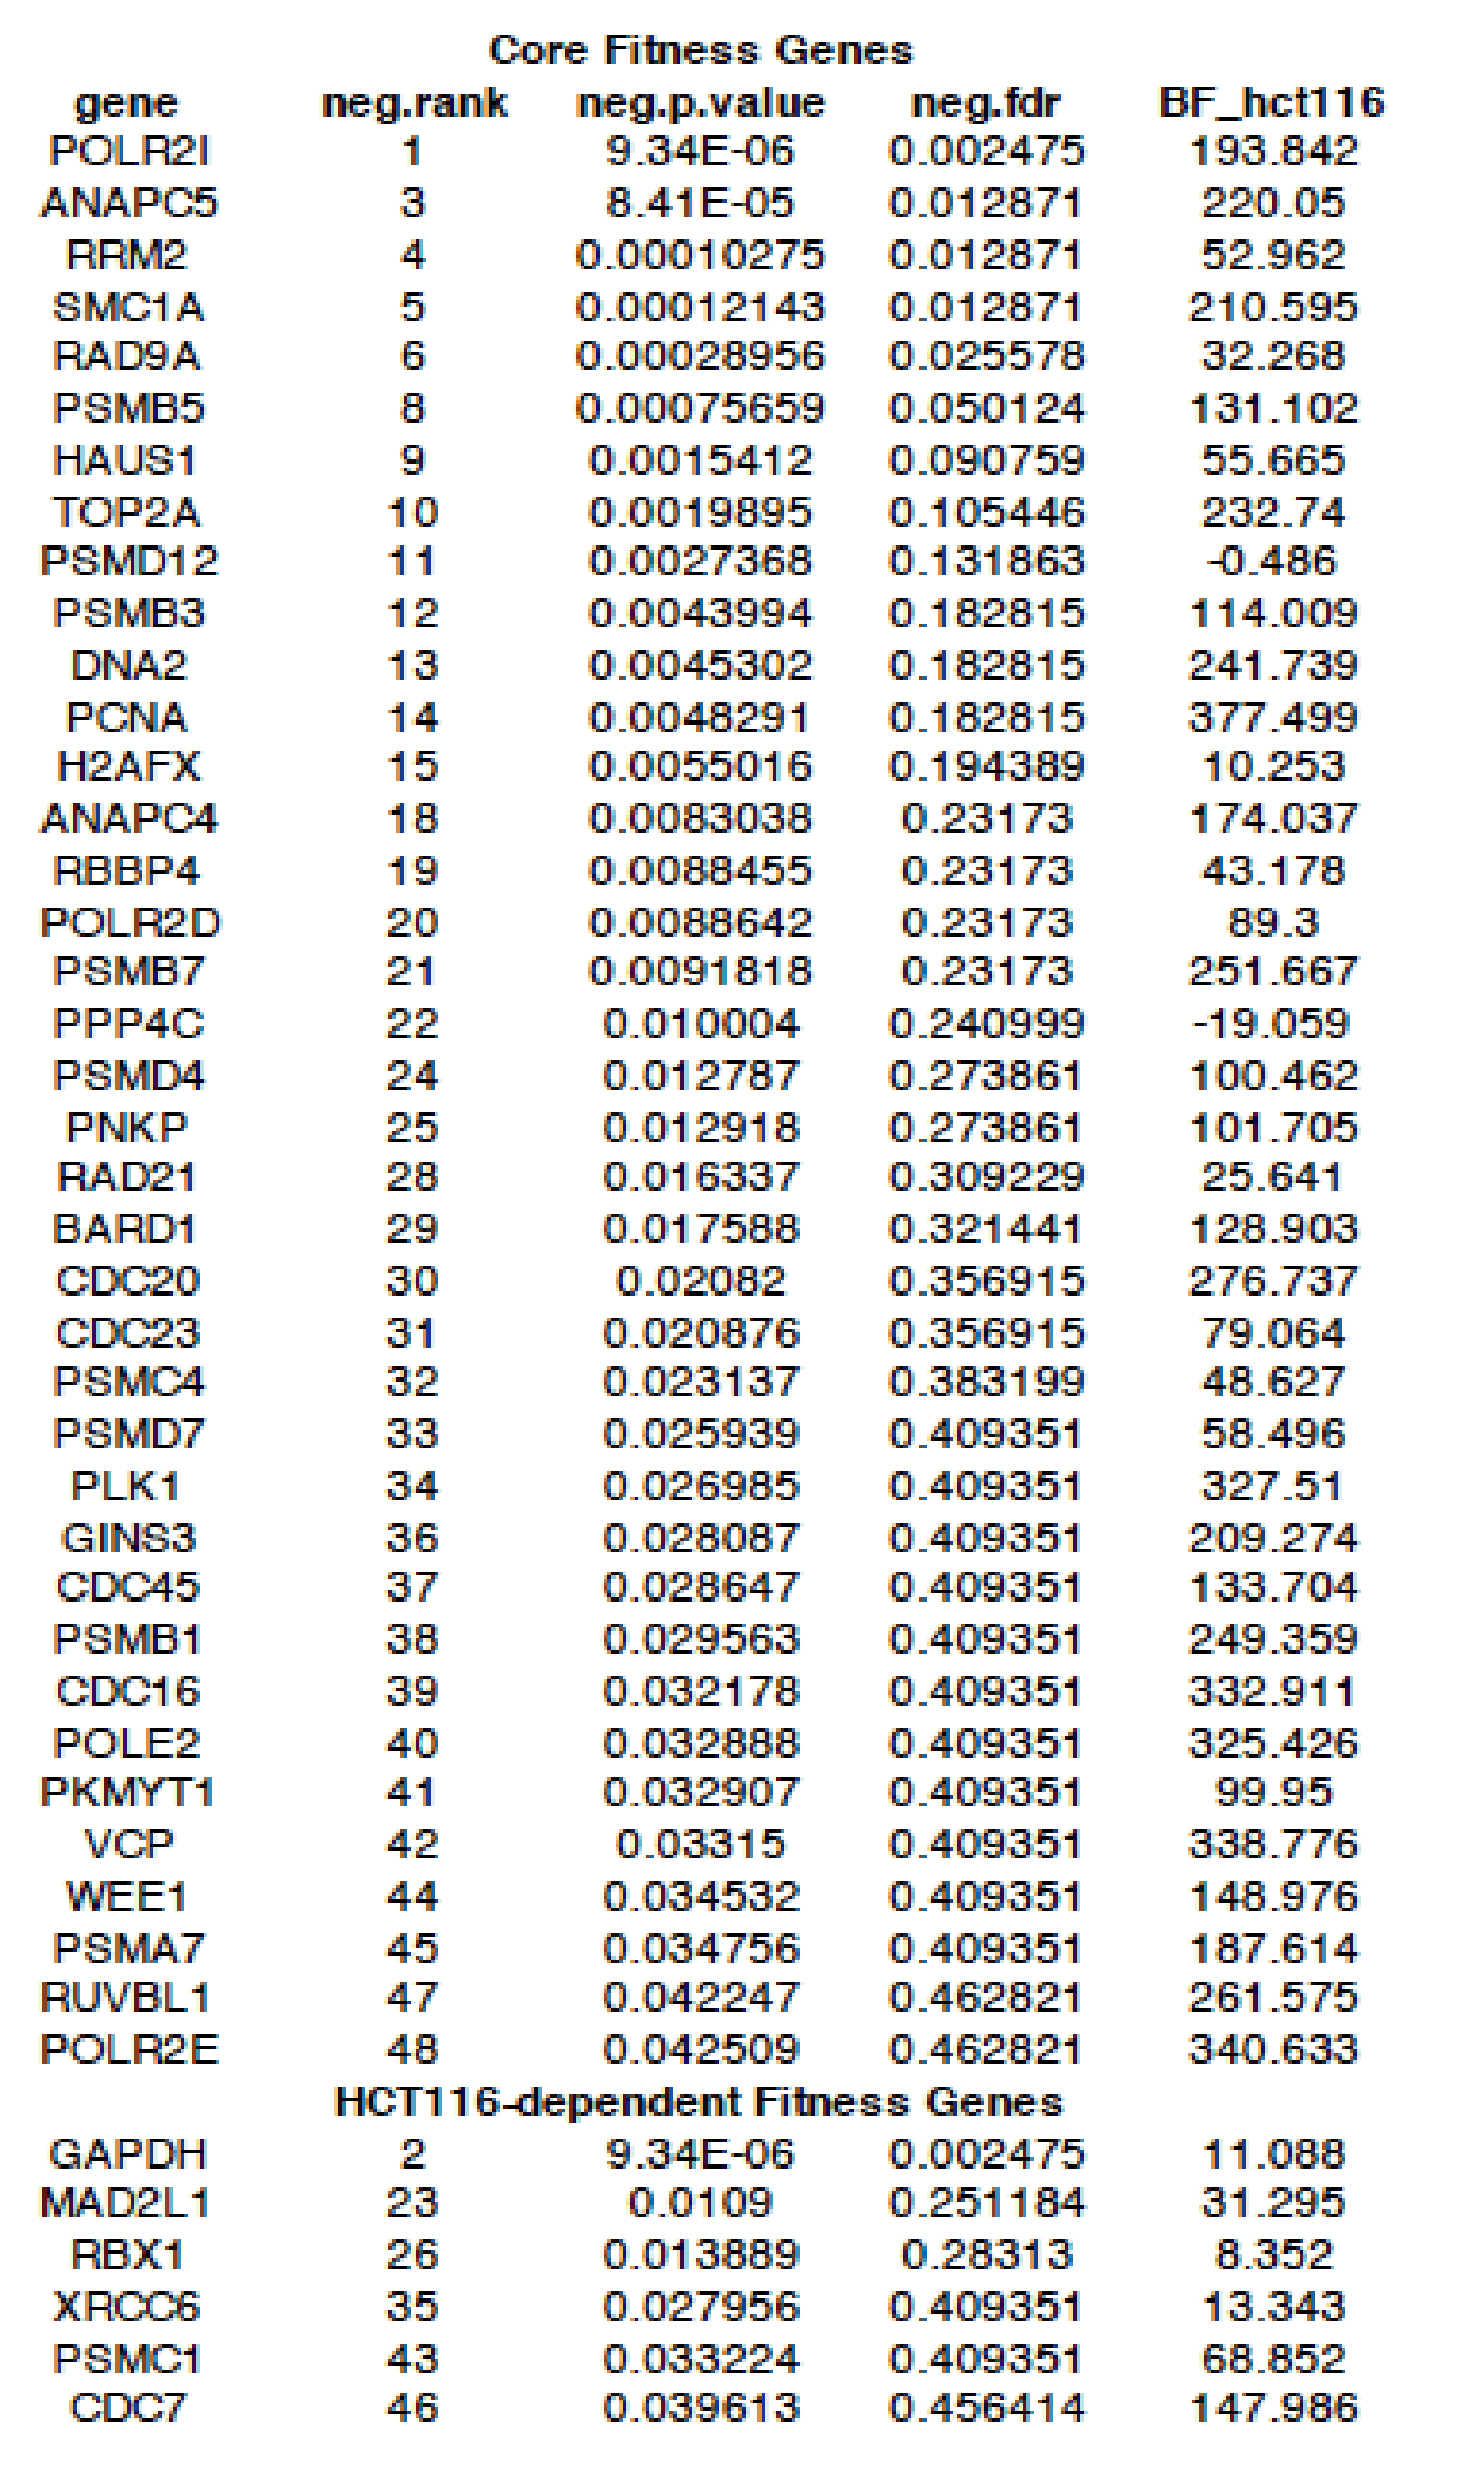
\includegraphics[width=0.8\textwidth]{supplement/tables/fitness_genes_depleted.png}
%\label{table:fitness_genes}
%\end{table}


%% Comparison of top 10% depleted genes with Hart et al.  fitness genes with Bayes factor (BF).

\begin{longtable}{>{\baselineskip=16pt}p{3cm} >{\baselineskip=16pt}p{1cm}  >{\baselineskip=16pt}p{3cm}   >{\baselineskip=16pt}p{3cm} >{\baselineskip=16pt}p{3cm}}
    \caption{Comparison of top 10\% depleted genes with Hart et al.  fitness genes with Bayes factor (BF).}
    \label{table:fitness_genes}\\
    \toprule
    %\renewcommand{\arraystretch}{0.18} 
Gene & Rank & p-value & FDR & BF (HCT116) \\
    \midrule
    \endfirsthead
    \multicolumn{5}{r}{\tablename\ \thetable\ -- \textit{Continued from previous page}} \\
    \toprule
    Gene & Rank & p-value & FDR & BF (HCT116) \\
    \midrule
    \endhead
    \bottomrule
    \multicolumn{5}{r}{\textit{Continued on next page}}
    \endfoot
    \bottomrule
    \endlastfoot
    %\renewcommand{\arraystretch}{0.4}
 \hline
 \multicolumn{5}{|c|}{Core fitness genes} \\
 \hline

POLR2I & 1 & 9.34E-06 & 0.002475 & 193.842 \\
ANAPC5 & 3 & 8.41E-05 & 0.012871 & 220.05 \\
RRM2 & 4 & 0.00010275 & 0.012871 & 52.962 \\
SMC1A & 5 & 0.00012143 & 0.012871 & 210.595 \\
RAD9A & 6 & 0.00028956 & 0.025578 & 32.268 \\
PSMB5 & 8 & 0.00075659 & 0.050124 & 131.102 \\
HAUS1 & 9 & 0.0015412 & 0.090759 & 55.665 \\
TOP2A & 10 & 0.0019895 & 0.105446 & 232.74 \\
PSMD12 & 11 & 0.0027368 & 0.131863 & -0.486 \\
PSMB3 & 12 & 0.0043994 & 0.182815 & 114.009 \\
DNA2 & 13 & 0.0045302 & 0.182815 & 241.739 \\
PCNA & 14 & 0.0048291 & 0.182815 & 377.499 \\
H2AFX & 15 & 0.0055016 & 0.194389 & 10.253 \\
ANAPC4 & 18 & 0.0083038 & 0.23173 & 174.037 \\
RBBP4 & 19 & 0.0088455 & 0.23173 & 43.178 \\
POLR2D & 20 & 0.0088642 & 0.23173 & 89.3 \\
PSMB7 & 21 & 0.0091818 & 0.23173 & 251.667 \\
PPP4C & 22 & 0.010004 & 0.240999 & -19.059 \\
PSMD4 & 24 & 0.012787 & 0.273861 & 100.462 \\
PNKP & 25 & 0.012918 & 0.273861 & 101.705 \\
RAD21 & 28 & 0.016337 & 0.309229 & 25.641 \\
BARD1 & 29 & 0.017588 & 0.321441 & 128.903 \\
CDC20 & 30 & 0.02082 & 0.356915 & 276.737 \\
CDC23 & 31 & 0.020876 & 0.356915 & 79.064 \\
PSMC4 & 32 & 0.023137 & 0.383199 & 48.627 \\
PSMD7 & 33 & 0.025939 & 0.409351 & 58.496 \\
PLK1 & 34 & 0.026985 & 0.409351 & 327.51 \\
GINS3 & 36 & 0.028087 & 0.409351 & 209.274 \\
CDC45 & 37 & 0.028647 & 0.409351 & 133.704 \\
PSMB1 & 38 & 0.029563 & 0.409351 & 249.359 \\
CDC16 & 39 & 0.032178 & 0.409351 & 332.911 \\
POLE2 & 40 & 0.032888 & 0.409351 & 325.426 \\
PKMYT1 & 41 & 0.032907 & 0.409351 & 99.95 \\
VCP & 42 & 0.03315 & 0.409351 & 338.776 \\
WEE1 & 44 & 0.034532 & 0.409351 & 148.976 \\
PSMA7 & 45 & 0.034756 & 0.409351 & 187.614 \\
RUVBL1 & 47 & 0.042247 & 0.462821 & 261.575 \\
POLR2E & 48 & 0.042509 & 0.462821 & 340.633 \\
 \hline
 \multicolumn{5}{|c|}{HCT116-dependent fitness genes} \\
 \hline
GAPDH & 2 & 9.34E-06 & 0.002475 & 11.088 \\
MAD2L1 & 23 & 0.0109 & 0.251184 & 31.295 \\
RBX1 & 26 & 0.013889 & 0.28313 & 8.352 \\
XRCC6 & 35 & 0.027956 & 0.409351 & 13.343 \\
PSMC1 & 43 & 0.033224 & 0.409351 & 68.852 \\
CDC7 & 46 & 0.039613 & 0.456414 & 147.986 \\

\end{longtable}


%\begin{table}
%\caption{sgRNA Sequences Used for Genetic Validation.}
%\centering
%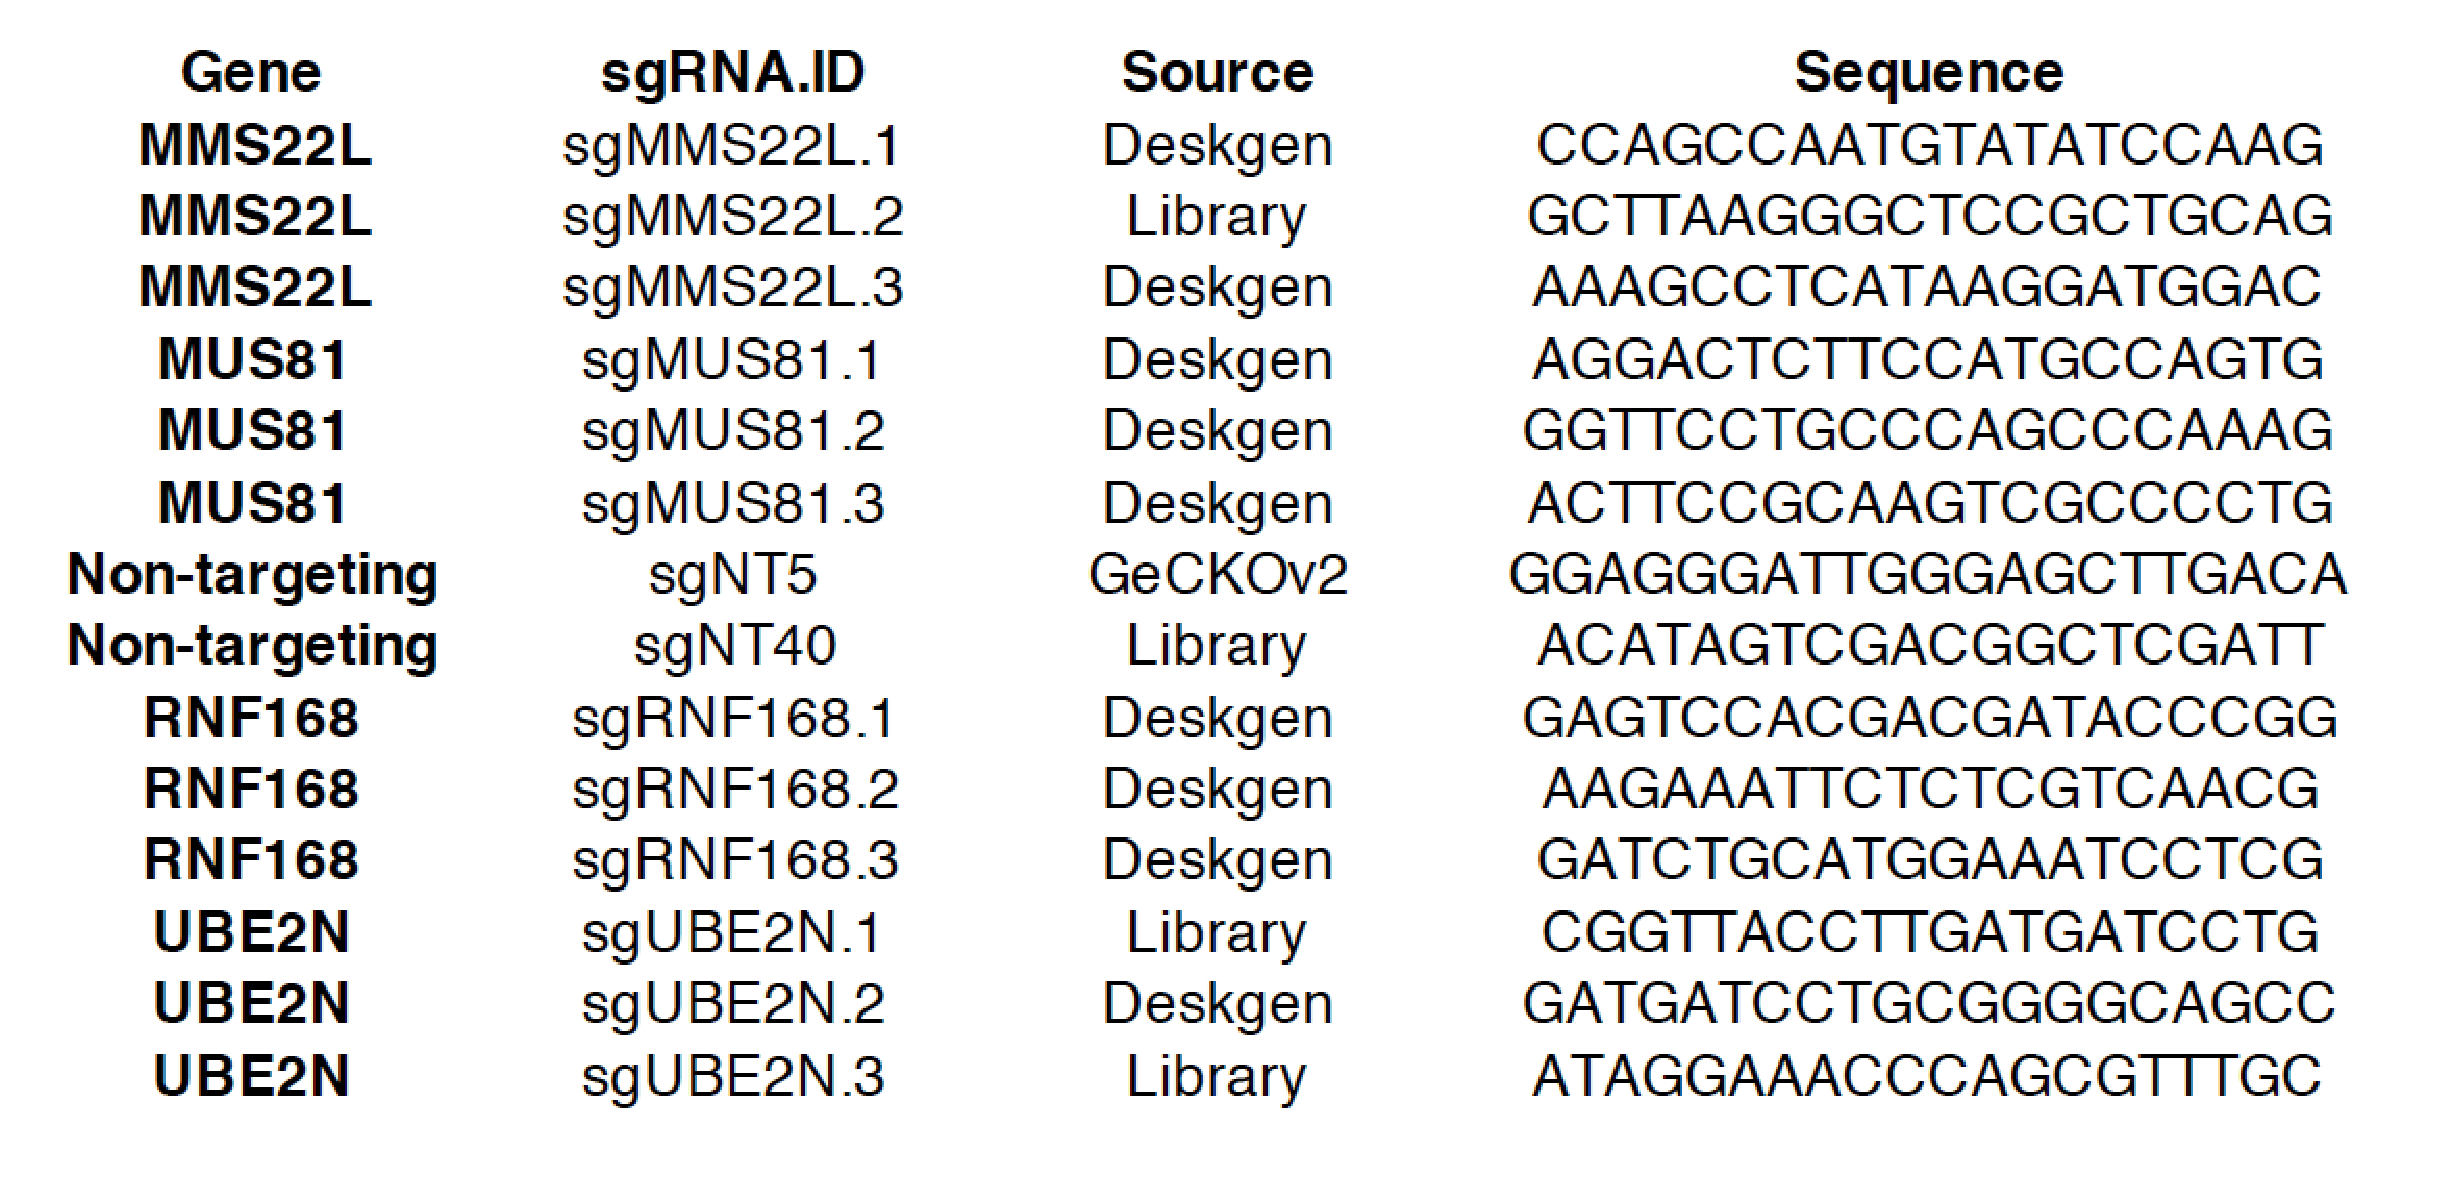
\includegraphics[width=1\textwidth]{supplement/tables/STable_sgRNA_sequences}
%\label{table:sgRNA_sequences}
%\end{table}

%% sgRNA sequences used for genetic validation table

\begin{longtable}{>{\baselineskip=22pt}p{4cm} >{\baselineskip=22pt}p{3cm}  >{\baselineskip=22pt}p{2cm} >{\baselineskip=22pt}p{6cm}}
    \caption{sgRNA sequences used for genetic validation.}
    \label{table:sgRNA_sequences}\\
    \toprule
    %\renewcommand{\arraystretch}{0.18} 
Gene & sgRNA ID & Source & Sequence \\
    \midrule
    \endfirsthead
    \multicolumn{4}{r}{\tablename\ \thetable\ -- \textit{Continued from previous page}} \\
    \toprule
    Gene & sgRNA ID & Source & Sequence \\
    \midrule
    \endhead
    \bottomrule
    \multicolumn{4}{r}{\textit{Continued on next page}}
    \endfoot
    \bottomrule
    \endlastfoot
    %\renewcommand{\arraystretch}{0.4}

MMS22L & sgMMS22L.1 & Deskgen & CCAGCCAATGTATATCCAAG \\
MMS22L & sgMMS22L.2 & Library & GCTTAAGGGCTCCGCTGCAG \\
MMS22L & sgMMS22L.3 & Deskgen & AAAGCCTCATAAGGATGGAC \\
MUS81 & sgMUS81.1 & Deskgen & AGGACTCTTCCATGCCAGTG \\
MUS81 & sgMUS81.2 & Deskgen & GGTTCCTGCCCAGCCCAAAG \\
MUS81 & sgMUS81.3 & Deskgen & ACTTCCGCAAGTCGCCCCTG \\
Non-targeting & sgNT5 & GeCKOv2 & GGAGGGATTGGGAGCTTGACA \\
Non-targeting & sgNT40 & Library & ACATAGTCGACGGCTCGATT \\
RNF168 & sgRNF168.1 & Deskgen & GAGTCCACGACGATACCCGG \\
RNF168 & sgRNF168.2 & Deskgen & AAGAAATTCTCTCGTCAACG \\
RNF168 & sgRNF168.3 & Deskgen & GATCTGCATGGAAATCCTCG \\
UBE2N & sgUBE2N.1 & Library & CGGTTACCTTGATGATCCTG \\
UBE2N & sgUBE2N.2 & Deskgen & GATGATCCTGCGGGGCAGCC \\
UBE2N & sgUBE2N.3 & Library & ATAGGAAACCCAGCGTTTGC \\


\end{longtable}


%\begin{table}
%\caption{Antibodies Used for Western Blots.}
%\centering
%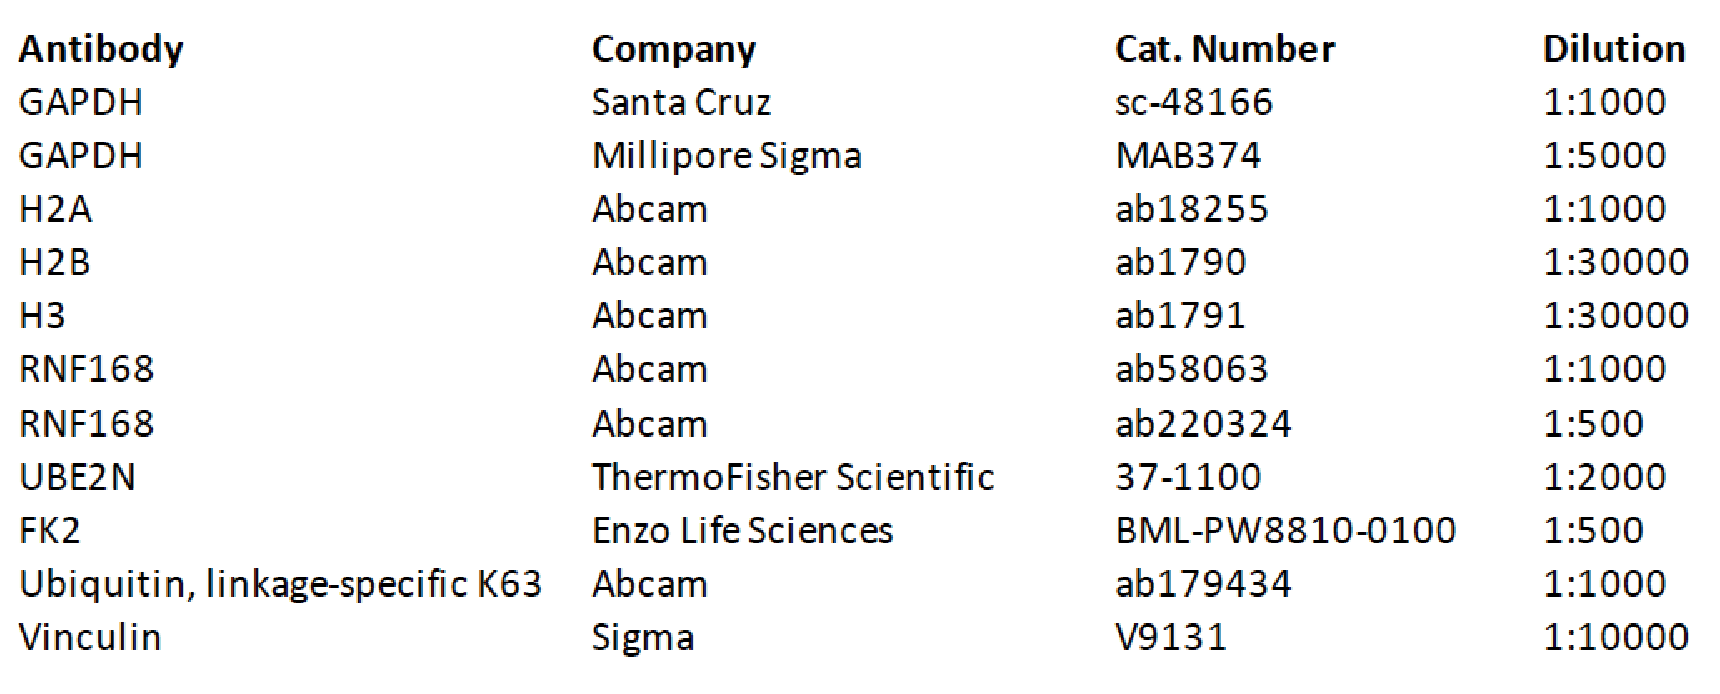
\includegraphics[width=1\textwidth]{supplement/tables/STable_Western_antibodies.png}
%\label{table:Western_antibodies}
%\end{table}


%% Antibodies Used for Western Blots

\begin{longtable}{>{\baselineskip=22pt}p{3.5cm} >{\baselineskip=22pt}p{5cm}  >{\baselineskip=22pt}p{5cm} >{\baselineskip=22pt}p{2cm}}
    \caption{Antibodies used for Western blots.}
    \label{table:Western_antibodies}\\
    \toprule
    %\renewcommand{\arraystretch}{0.18} 
Antibody & Company & Catalogue number & Dilution \\
    \midrule
    \endfirsthead
    \multicolumn{4}{r}{\tablename\ \thetable\ -- \textit{Continued from previous page}} \\
    \toprule
    Antibody & Company & Catalogue number & Dilution \\
    \midrule
    \endhead
    \bottomrule
    \multicolumn{4}{r}{\textit{Continued on next page}}
    \endfoot
    \bottomrule
    \endlastfoot
    %\renewcommand{\arraystretch}{0.4}

GAPDH & Santa Cruz & sc-48166  & 1:1000 \\
GAPDH & Millipore Sigma & MAB374 & 1:5000 \\
H2A & Abcam & ab18255 & 1:1000 \\
H2B & Abcam & ab1790 & 1:30000 \\
H3 & Abcam & ab1791 & 1:30000 \\
RNF168 & Abcam & ab58063 & 1:1000 \\
RNF168 & Abcam & ab220324 & 1:500 \\
UBE2N & ThermoFisher Scientific & 37-1100 & 1:2000 \\
FK2 & Enzo Life Sciences & BML-PW8810-0100 & 1:500 \\
Ubiquitin, linkage-specific K63 & Abcam & ab179434 & 1:1000 \\
Vinculin & Sigma & V9131 & 1:10000 \\

\end{longtable}






